%%%%%%%%%%%%%%%%%%%%%%%%%%%%%%%%%%%%%%%%%%%%%%%%%%%%%%%%%%%%%%%%%%%%%%%%
% 3. エレベータ利用状況可視化システム
%%%%%%%%%%%%%%%%%%%%%%%%%%%%%%%%%%%%%%%%%%%%%%%%%%%%%%%%%%%%%%%%%%%%%%%%
\section{A System for Visualizing Elevator Usage}

In this chapter, we explain the system diagram Figure \ref{fig:system} for visualizing the number of people in the elevator and the number of people on each floor.

% システム要件
\subsection{System Requirement}

To realize this system, the following requirements are necessary.

\begin{quote}
  \begin{itemize}
    \item Requirement 1: Obtain the number of people in the elevator and the status of the elevator hall on each floor.
    \item Requirement 2: Visualization of the information obtained in Requirement 1 for elevator users
  \end{itemize}
\end{quote}

% 図:システム2
\begin{figure}[t]
  \begin{center}
    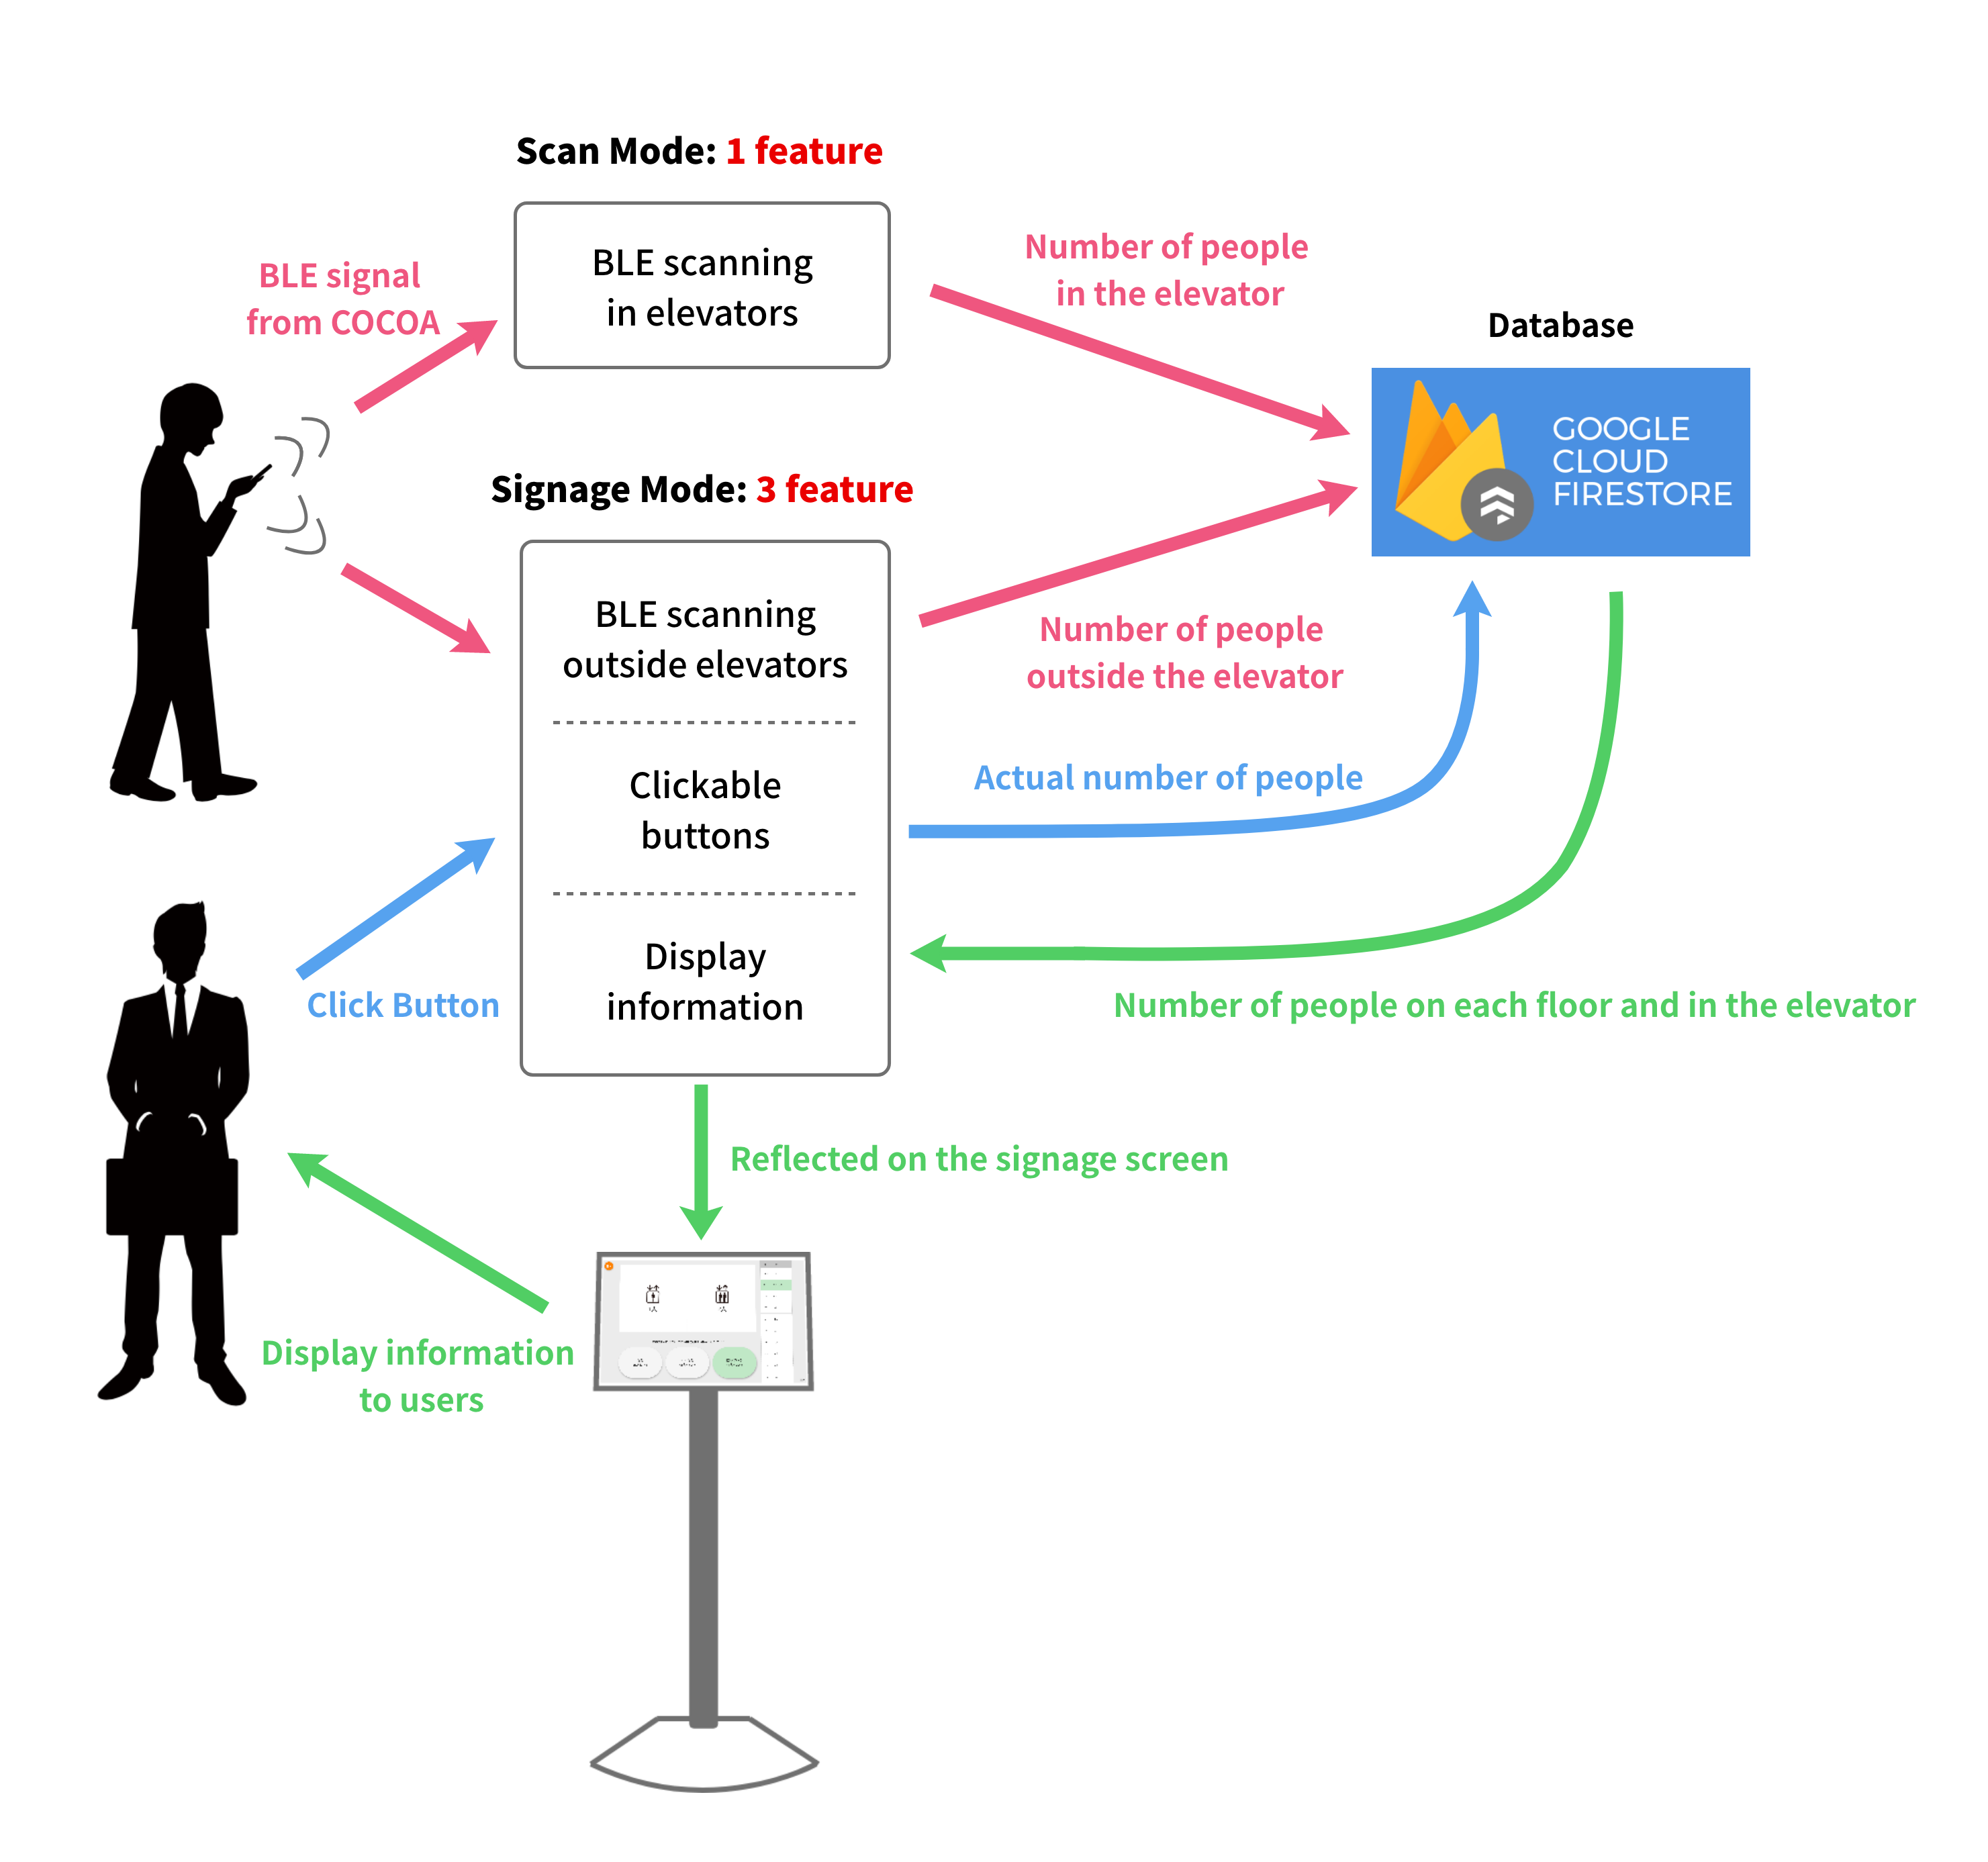
\includegraphics[clip,  width=1.0\hsize]{img/system2.png}
    \caption{System configuration}
    \label{fig:system2}
  \end{center}
\end{figure}

% 図:アプリケーションの画面
\begin{figure}[t]
  \begin{center}
    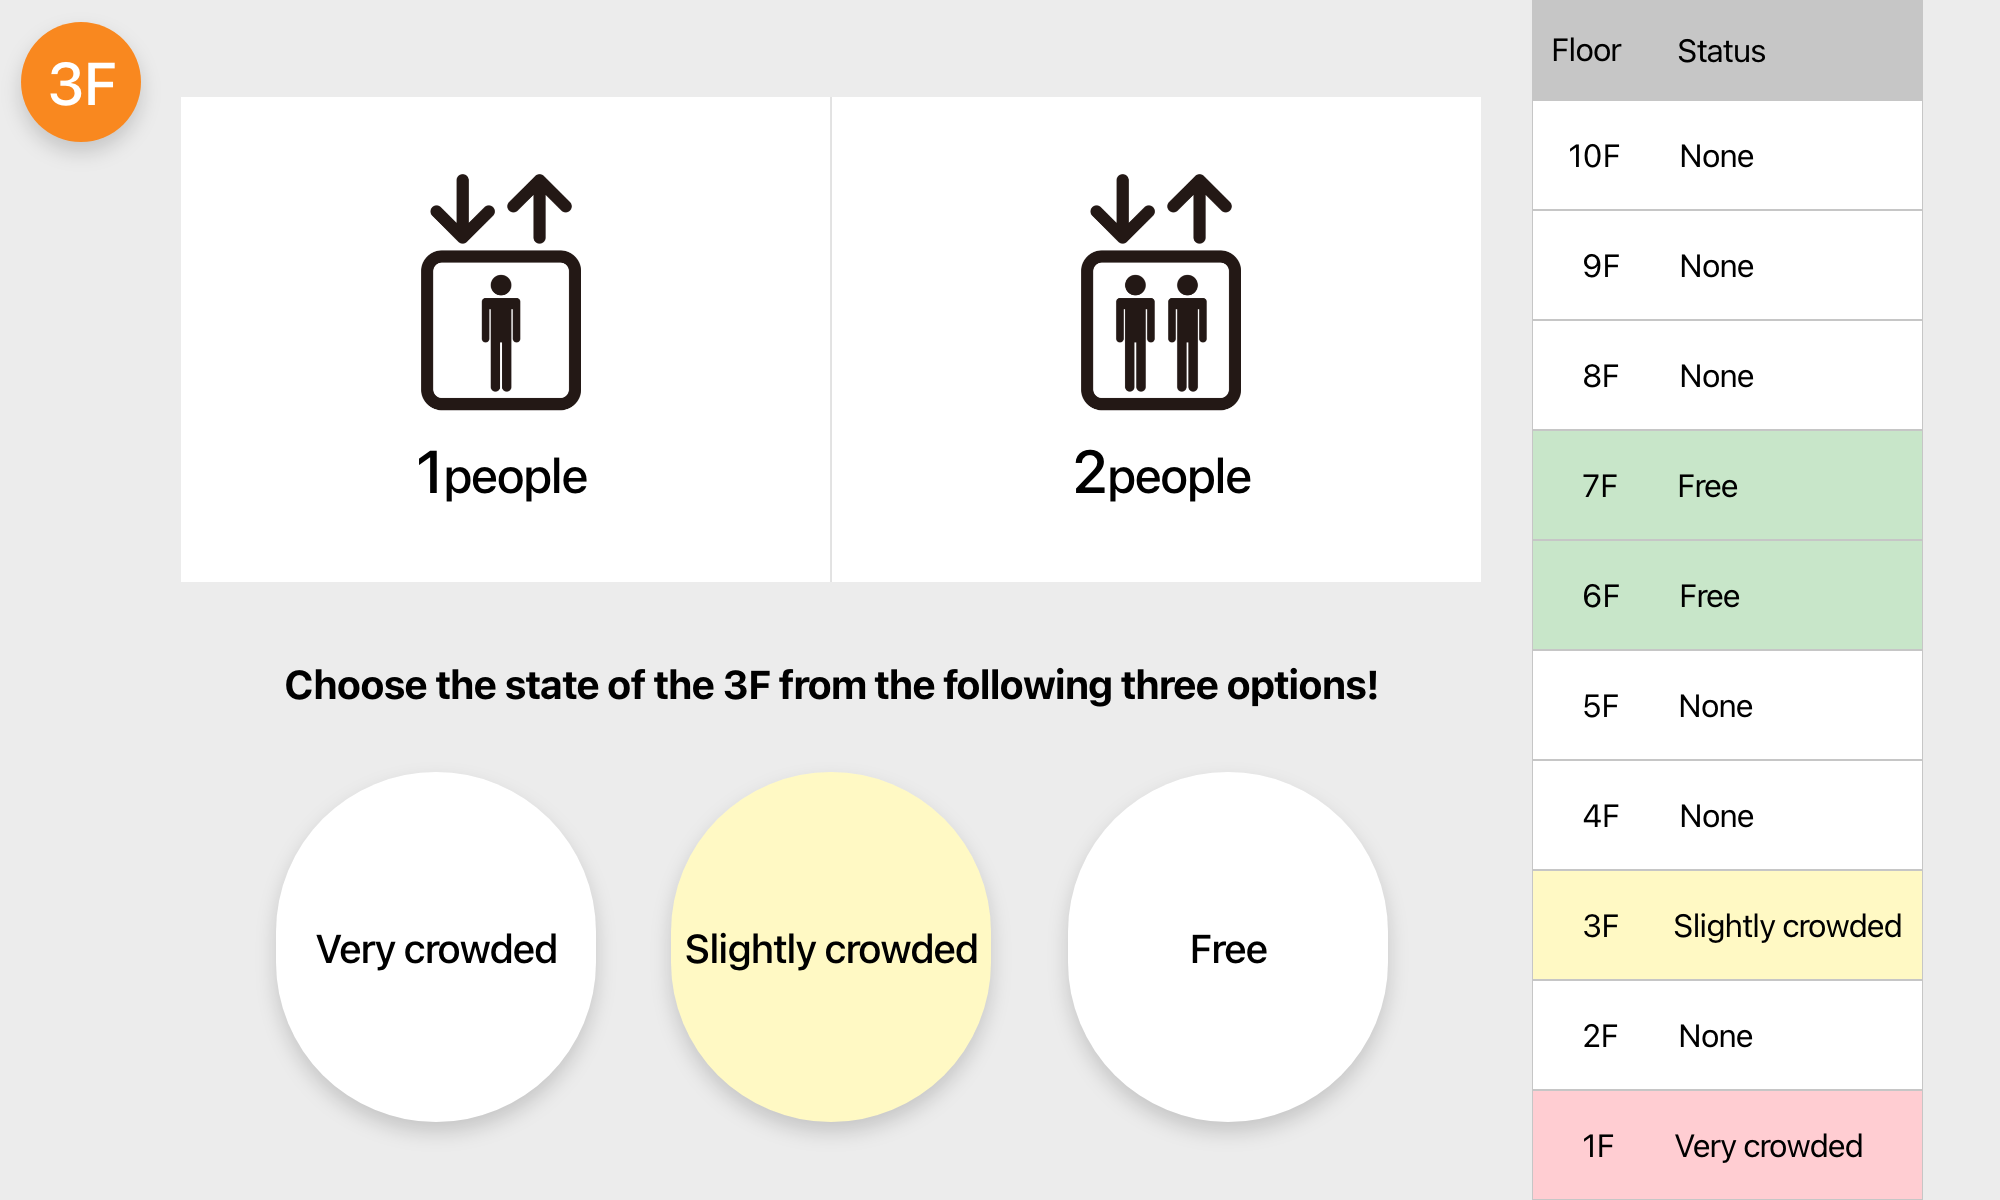
\includegraphics[clip,  width=1.0\hsize]{img/application_sceen.png}
    \caption{Application screen}
    \label{fig:application_sceen}
  \end{center}
\end{figure}

% 図:九州大学伊都キャンパスウエスト2号館 エレベータ内
\begin{figure}[t]
  \begin{center}
    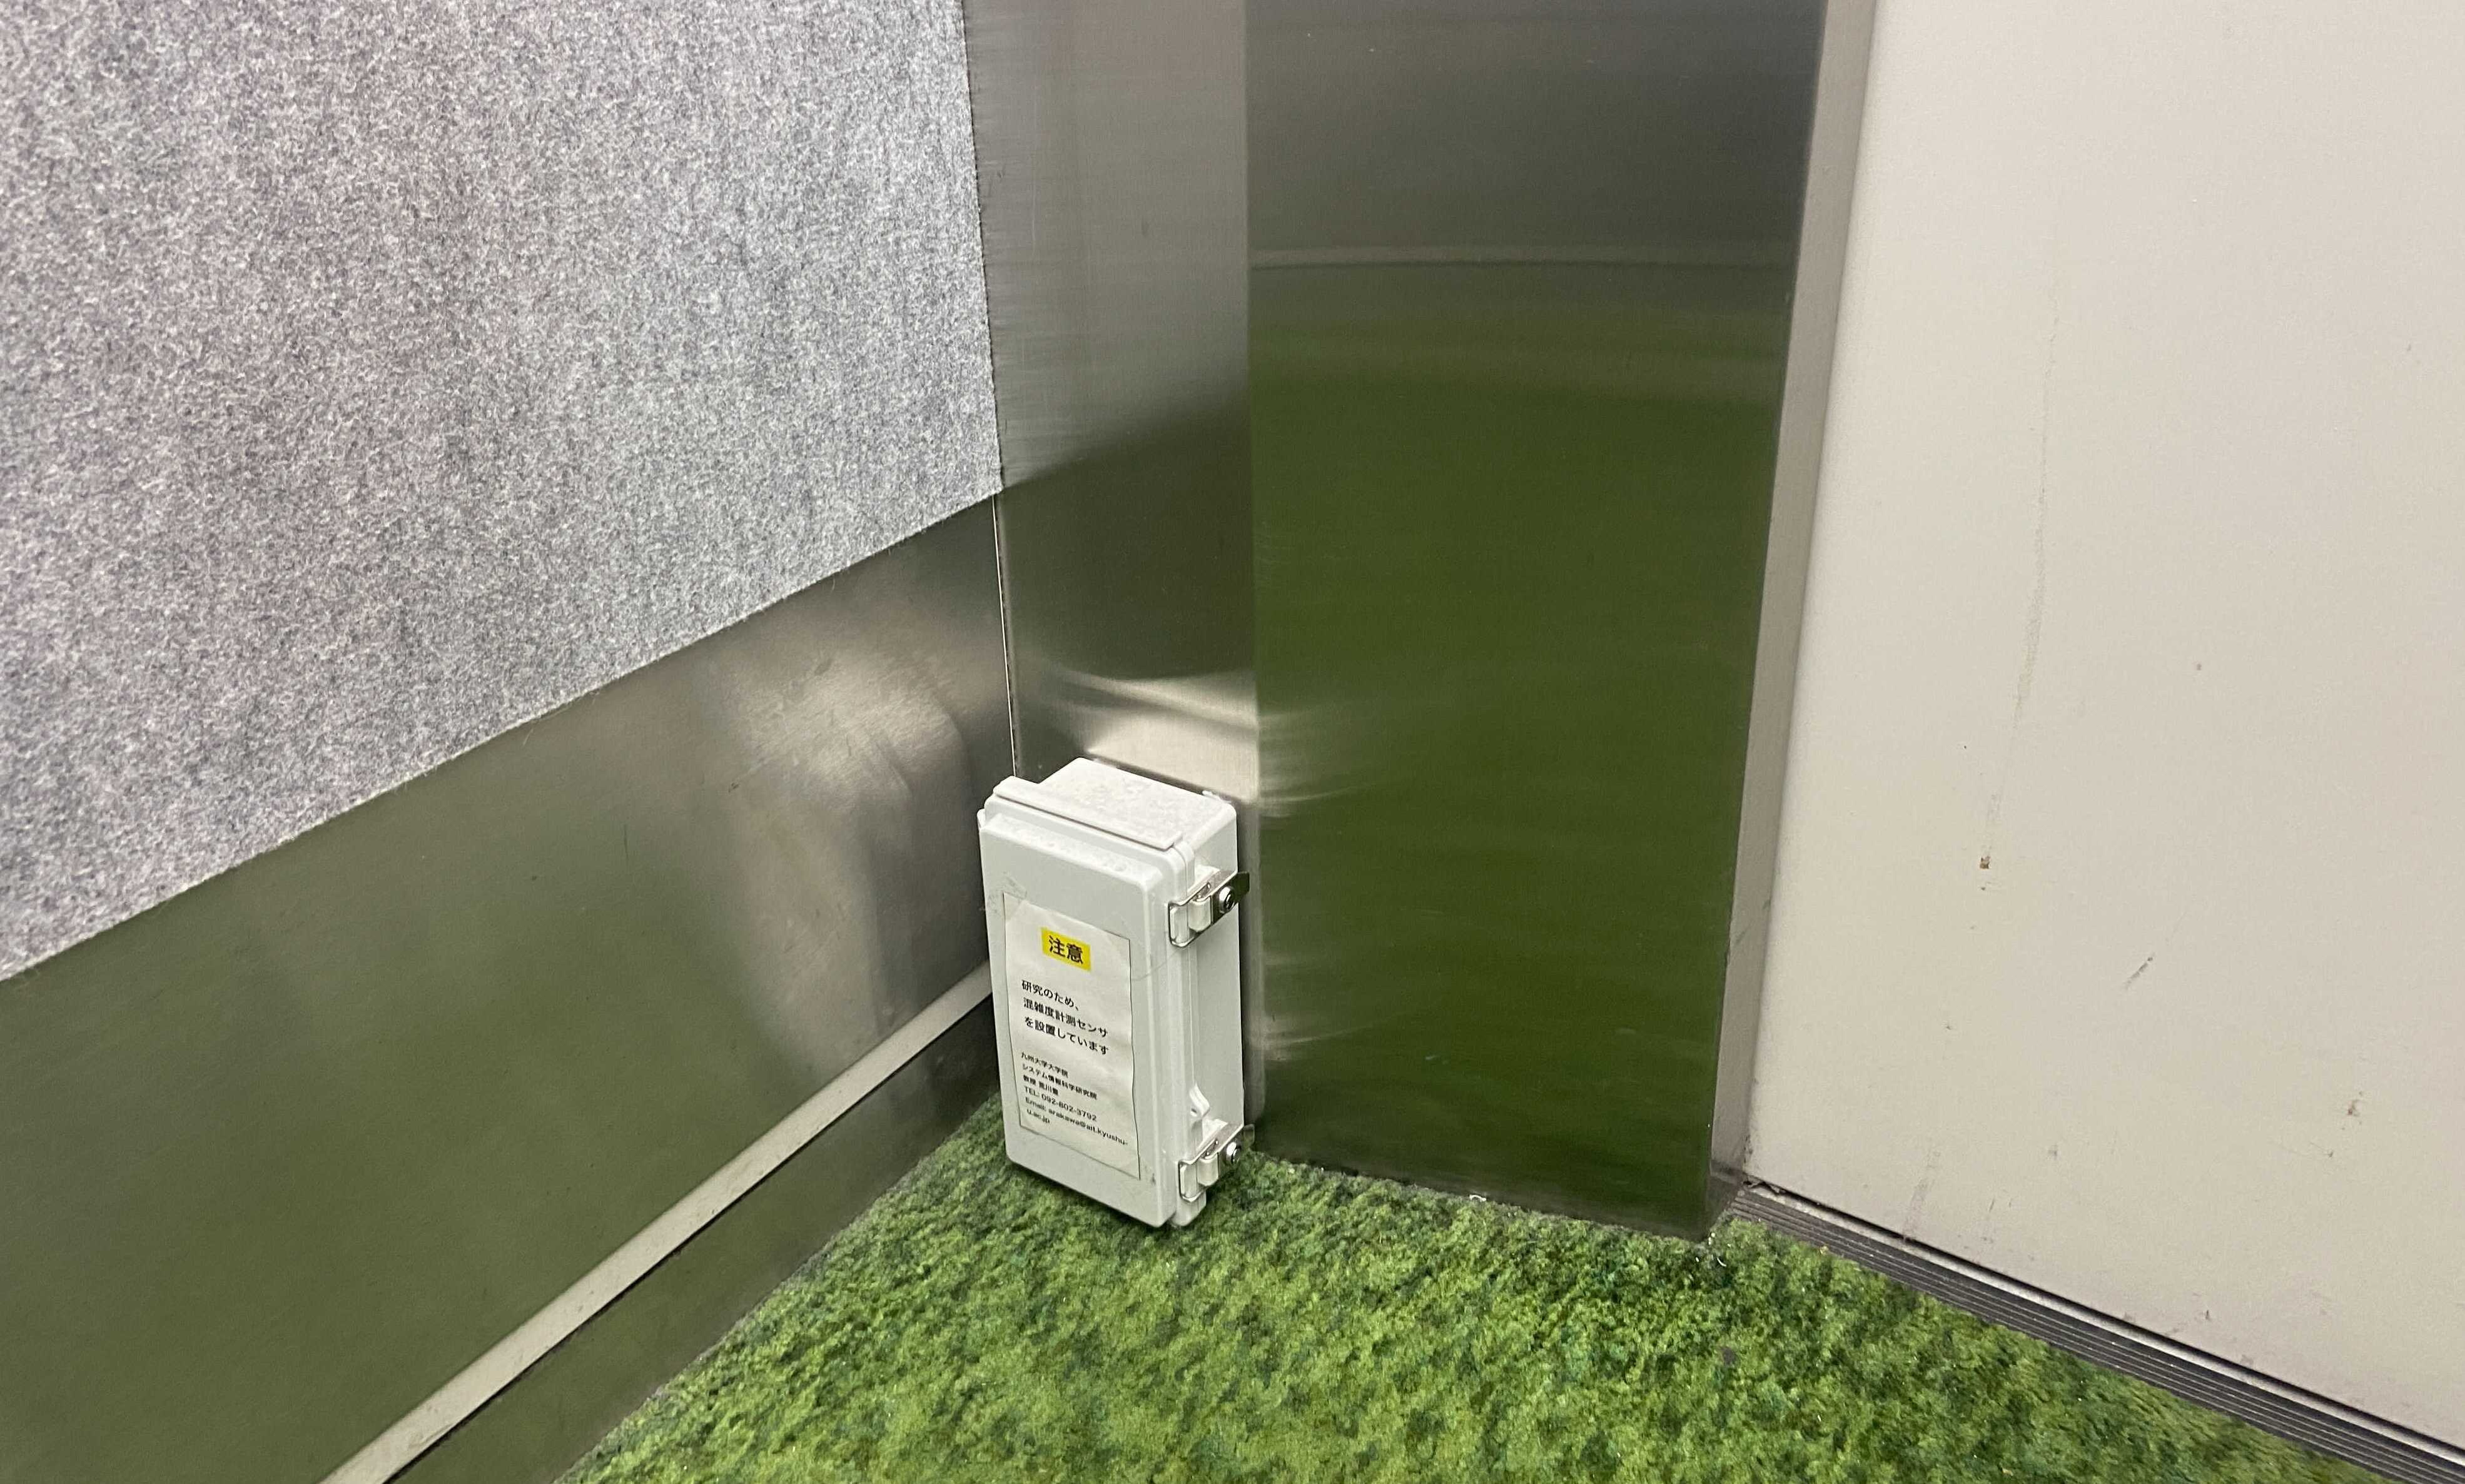
\includegraphics[clip,  width=1.0\hsize]{img/kyudai_west2_elevator_inside.jpg}
    \caption{Installation of smart phones in elevators}
    \label{fig:kyudai_west2_elevator_inside}
  \end{center}
\end{figure}

% 図:九州大学伊都キャンパスウエスト2号館9F
\begin{figure}[t]
  \begin{center}
    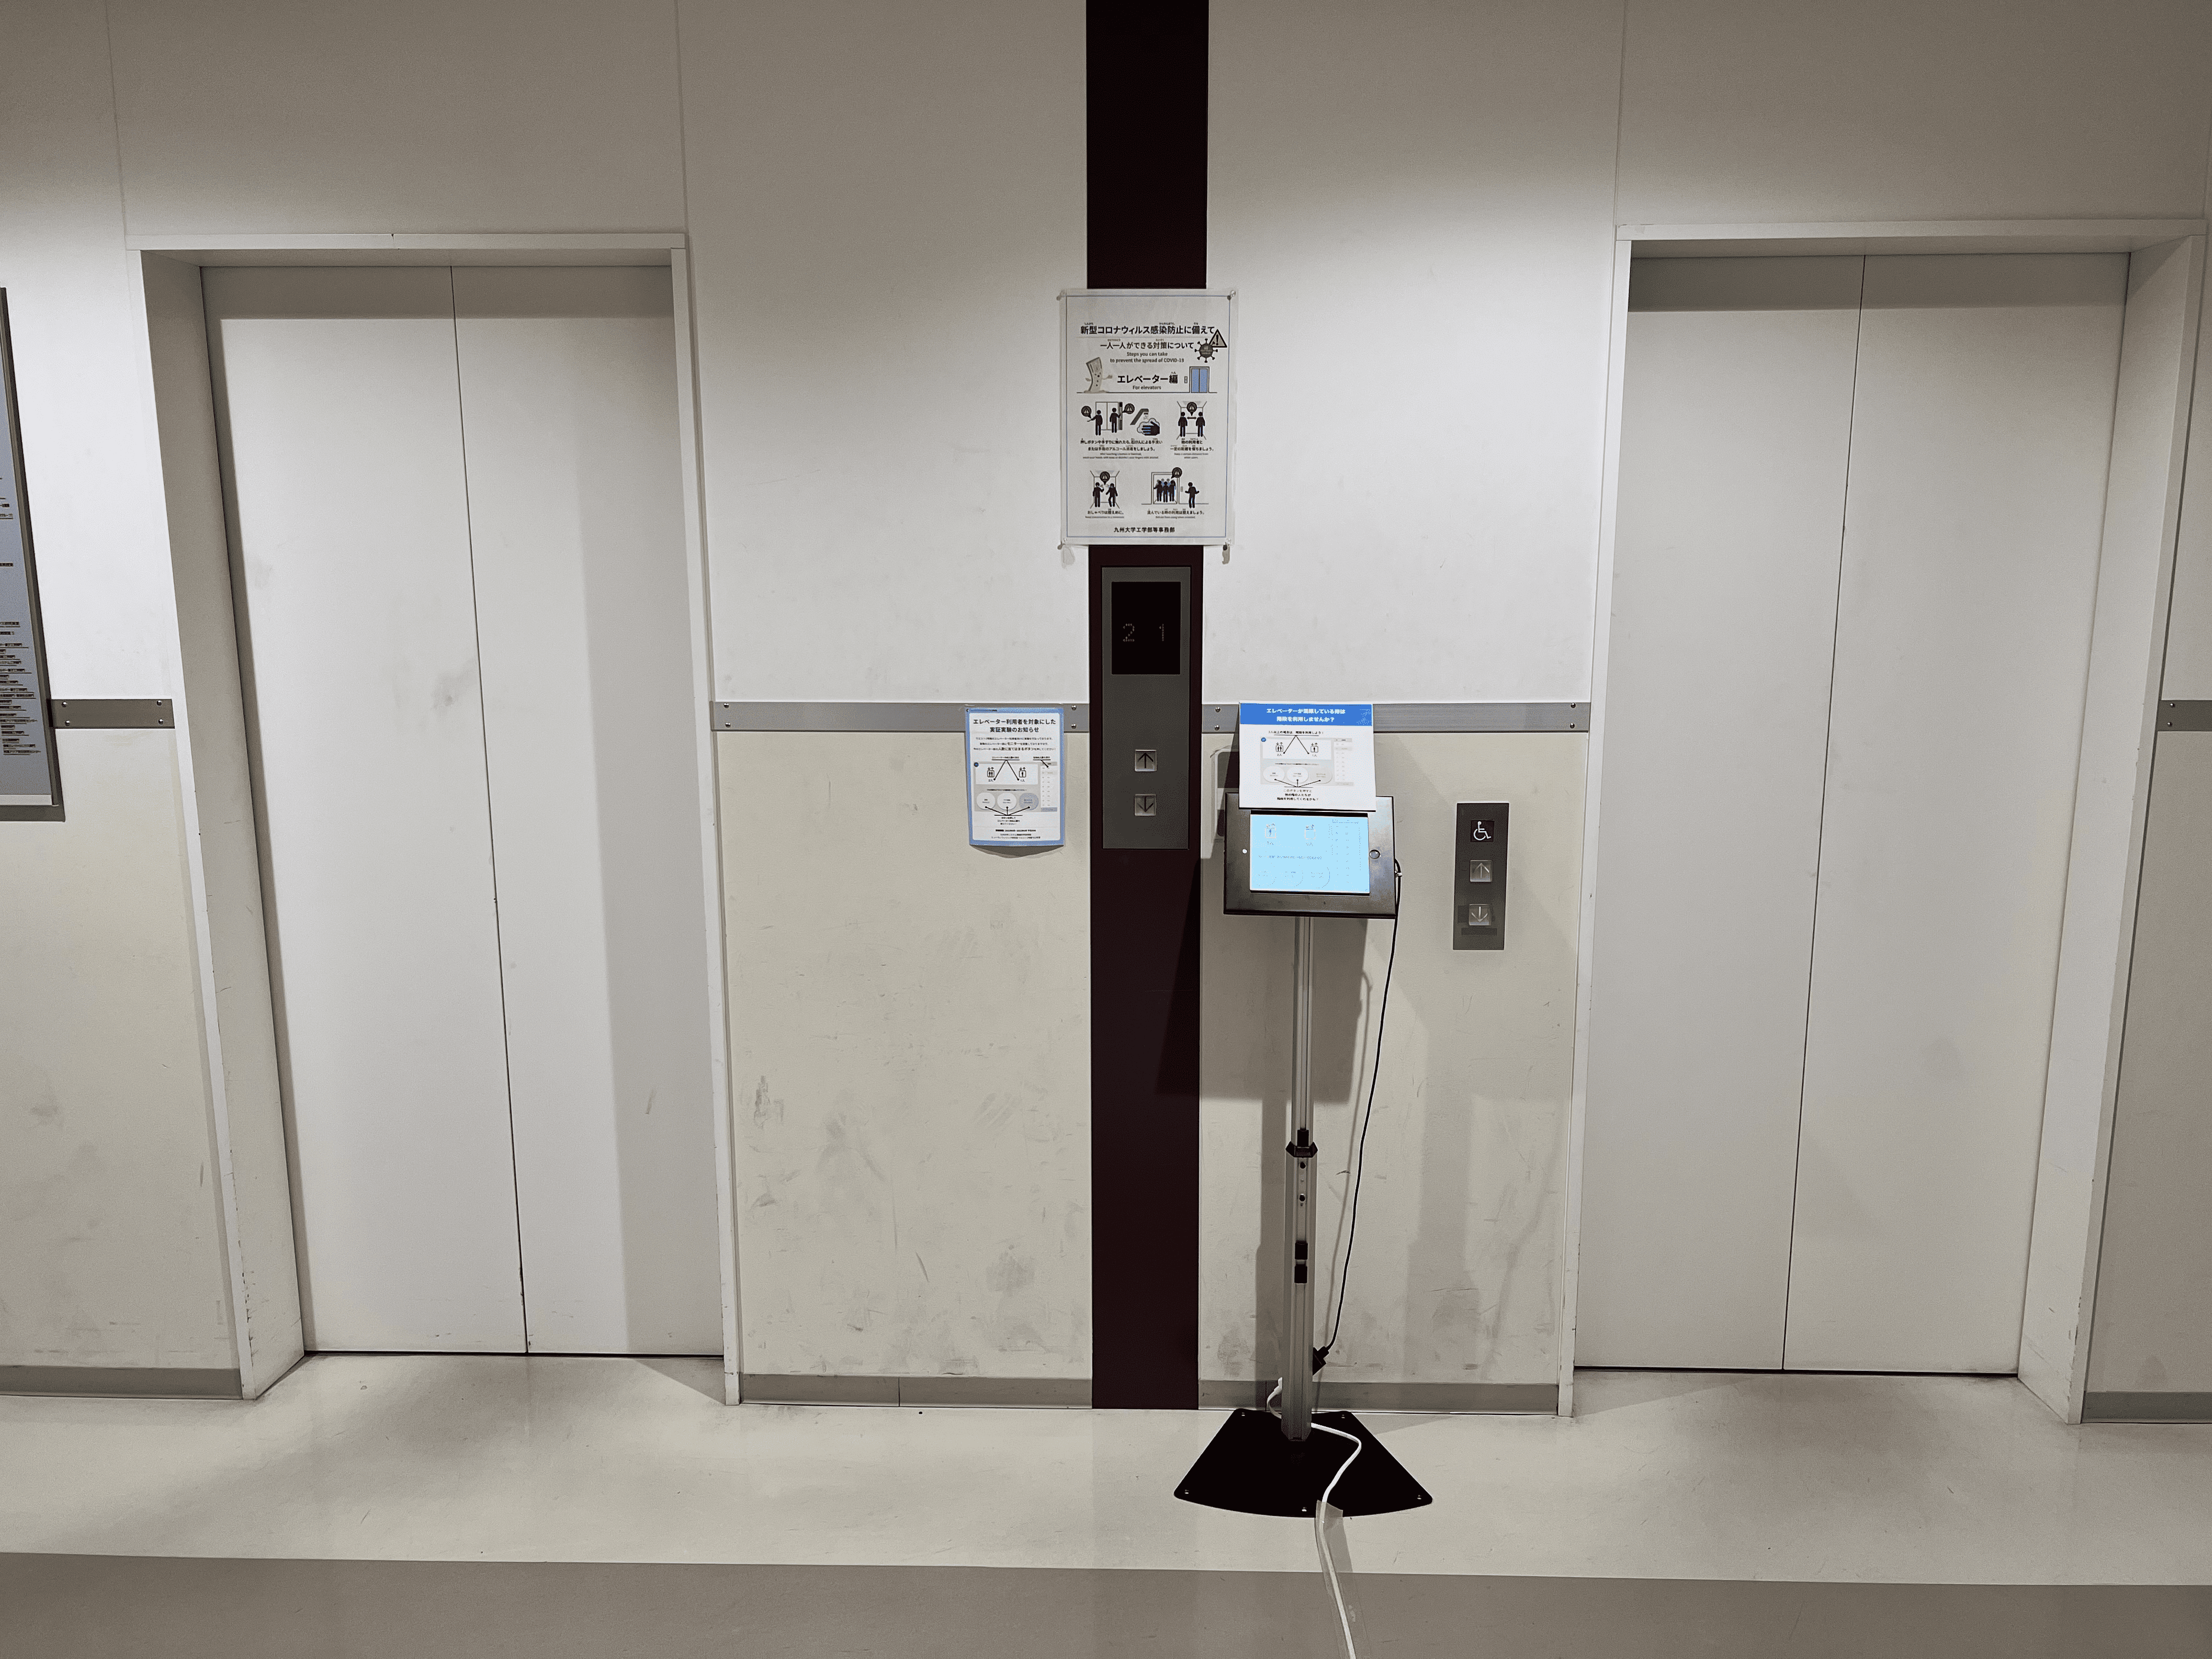
\includegraphics[clip,  width=1.0\hsize]{img/kyudai_west2_elevator.png}
    \caption{Installation of tablets in the elevator hall.}
    \label{fig:kyudai_west2_elevator}
  \end{center}
\end{figure}

% システム実装
\subsection{System Implementation}

The configuration of this system is shown in Figure \ref{fig:system2}. The reason why we are using a smartphone as the sensor to be installed in the elevator is because we thought that an inexpensive smartphone would be suitable as a platform with built-in WiFi/BLE/LTE and a battery. The application developed in this study has a scan mode and a signage mode in one application, and can be used by simply switching between these two modes. Maintenance costs have been reduced by unifying the apps for smartphone used as sensors in elevator and tablet for displaying information. The scan mode is for smartphones installed inside the elevator (Figure \ref{fig:kyudai_west2_elevator_inside}), and only the BLE scanning function can be used. Since the basic power supply is not available in the elevator, we reduced the functions to the minimum to enable the system to operate continuously for about a day without power supply. In the signage mode, the system is designed for a tablet installed in the elevator hall (Figure \ref{fig:kyudai_west2_elevator}), and in addition to the BLE scanning function, it has a feedback function with three levels of buttons and a function to display the number of people in the elevator and the degree of congestion on each floor. In addition to the BLE scan function, this mode provides a feedback function with three levels of buttons, and a function to display the number of people in the elevator and the congestion level on each floor (Figure \ref{fig:application_sceen}). This mode basically assumes that the power can be supplied and that the lights are always on. For the implementation of the application, a framework called Flutter is used.

This section describes the technical description. First of all, in order to realize Requirement 1, we detect BLE signals of -70 dBm or higher and count the number of people. However, if all BLE signals are used to count the number of people, the problem of duplicate counting of people who own multiple devices, such as Bluetooth earphones and smartphones, will occur. Therefore, we filter out only the BLE signals of COCOA to count only smartphone devices. Therefore, only the BLE signal of COCOA is filtered so that only smartphone devices are counted. The BLE standard for COCOA has been determined worldwide, and it is possible to filter only the signals of COCOA based on the values of \cite{cocoa_ble} and ServiceUUID. However, there is a problem that the COCOA signal transmitted from the Android terminal is weak and cannot be detected if the distance is too far, but this method is used in this system because the distance between the sensor and the Android terminal is close since the elevator is a narrow and closed space. For the database, we use Cloud Firestore, and all the BLE signal data is stored in Cloud Firestore.

Next, in order to realize Requirement 2, the number of people in the elevator and the congestion level of each floor are obtained from Cloud Firestore and displayed on the tablet screen (Figure \ref{fig:application_sceen}). In addition, in order to ask users to input the current status of the floor, the system displays the following information: crowded (more than 6 people), slightly crowded (3 people $\sim$ 5 people), and empty (1 person $\sim$ 2 people). Unlike the inside of an elevator, the elevator hall is not a shielded space, and unintended signals may be counted, so we have adopted the method of asking the users to press the buttons themselves.
